\chapter{Results and Performance Analysis}
\section{Introduction}
The format of this chapter is as follows:
\begin{itemize}
  \item Discussion of Verification results and implications
  \item Discussion of GPU OSB performance and line / device scalability
  \item Discussion of GPU ISB performance and line / device scalability
\end{itemize}

From the results of solution development, it's clear that while computational accuracy has been a casualty of the move to GPU, speed has been greatly improved. This section attempts to quantify this speed-up and the factors that contribute and detract from it.

In order to quantify this speed-up, it is important to look at three main factors; runtime execution in terms of bundle size, runtime execution in terms of multiple device use, and comparative speed-up characteristics compared to CPU execution.

These results will be presented graphically and in tabular format.

\section{OSB GPU Performance and Scalability}
\subsection{Runtime vs Bundle Size vs Device Count}
\begin{figure}[h!]
\centering
  \begin{tabularx}{0.6\textwidth}{|c|X|c|c|c|c|}
  \hline
  &CPU time&\multicolumn{4}{|c|}{GPU Count runtime (s)}\\
  N&&1&2&3&4\\\hline
  2&73.881&9.159&8.147&9.036&9.097\\
  3&651.977&18.737&13.523&12.851&13.100\\
  4&3118.691&334.820&175.373&122.746&98.096\\
  5&16597.065&6320.587&3175.932&2136.499&1605.589\\\hline
  \end{tabularx}
\caption{GPU Performance analysis of OSB: execution times against bundle sizes \& device counts}
\label{tab:OSBTable}
\end{figure}

\begin{figure}[h!]
  \centering
  \subfloat[Analysis of Execution speed vs N-GPUs]{\label{fig:GPU-OSB-multicomp-GPU}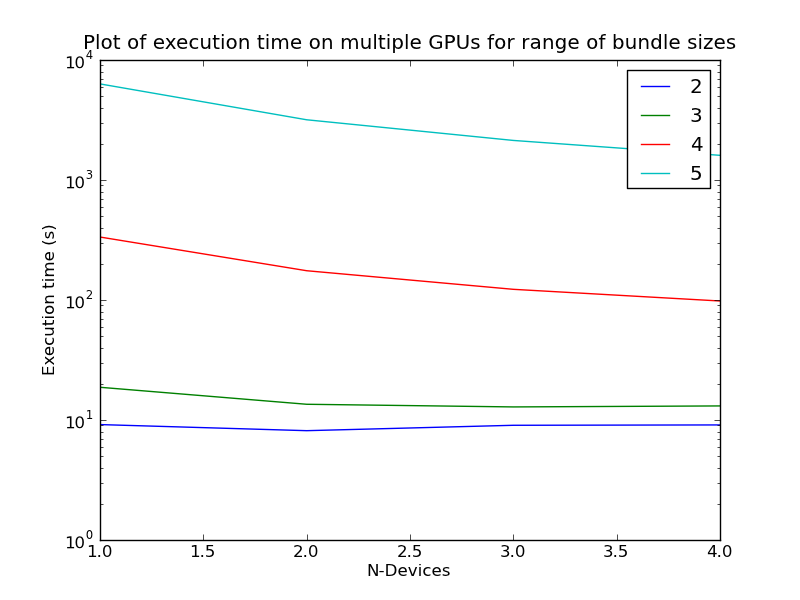
\includegraphics[width=0.5\textwidth,keepaspectratio=true]{cum-results/raw_results/OSB-gpucompare.png}}
  \subfloat[Analysis of Execution speed vs N-Lines]{\label{fig:GPU-OSB-multicomp-lines}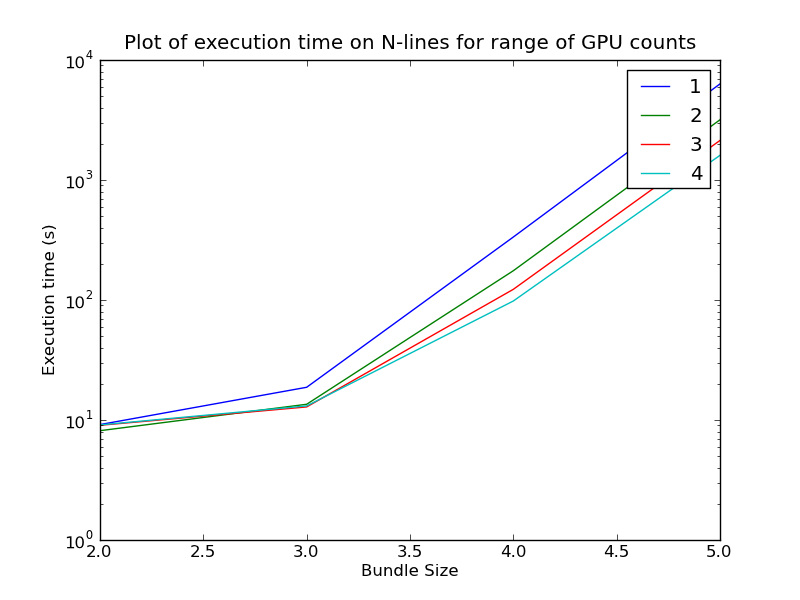
\includegraphics[width=0.5\textwidth,keepaspectratio=true]{cum-results/raw_results/OSB-linecompare.png}}
  \\
  \caption{Graphs of OSB Multi-GPU performance}
  \label{fig:GPU-OSB-multicomp}
\end{figure}

These results largely reflect what would be expected of parallel performance behaviour, specifically Amdahl's Law; as the number of parallel execution units is increased, the execution time asymptotically drops to a level beyond which increased parallelism is fruitless. This is particularly clear in figure \ref{fig:GPU-OSB-multicomp-GPU} for the lowest bundle sizes, where it appears that after using only two devices, no further gains are attained. This can easily be explained given the relatively small workload experiences at these sizes of bundle. As the bundle size is increased, the increase in workload allows multiple devices to be more useful, as the execution time of one devices work packets overtakes the memory transfer and serial algorithmic overheads.

Also indicated in both charts is that the two-device results indicate a 'sweet spot'; where the most speed-up is attained for the least device-count. For larger bundle counts, this is not applicable, as the workload is significant enough to allow for efficient work allocation taking advantage of all devices.

It is also evident from these results that this form of parallelism cannot avoid the computation-explosion inherent in OSB. 
\subsection{Relative Speed-up}
In order to assess the viability of using GPU for this application, it's important to put these results in the context of serial calculations.

To do so, the Parallel Speed-up ratio is applied to the results, such that \(S_p=\frac{T_1}{T_p}\) where \(T_1\) is the execution time for a serial instance, and \(T_p\) is the parallel execution time. This is a particularly difficult relationship to apply to GPU; should one count each device as a parallelisation unit, or each SM on each device? This is not so much a problem when calculating the pure speed up of an application, as the number of processing units is not a factor, but is a serious consideration when looking at the parallel efficiency, \(E_p=\frac{S_p}{P}\) where \(P\) is the number of parallel processing units. 

Initially looking purely at the parallel speed-up attained, the results speak for themselves.
\begin{figure}[h!]
\centering
\subfloat[OSB Parallel Speedup]{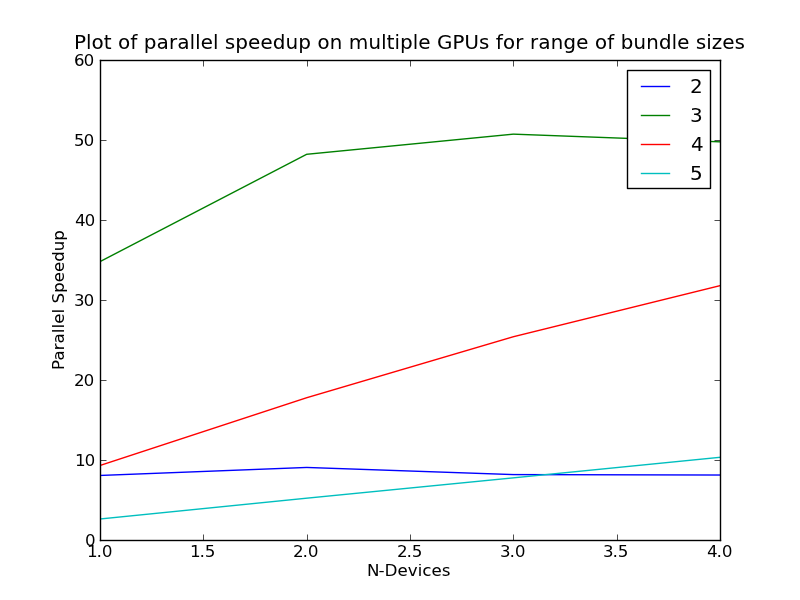
\includegraphics[width=0.45\textwidth,keepaspectratio=true]{cum-results/raw_results/OSB-gpuspeedup.png} \label{fig:GPU-OSB-speedup}}
\subfloat[OSB Parallel Efficiency]{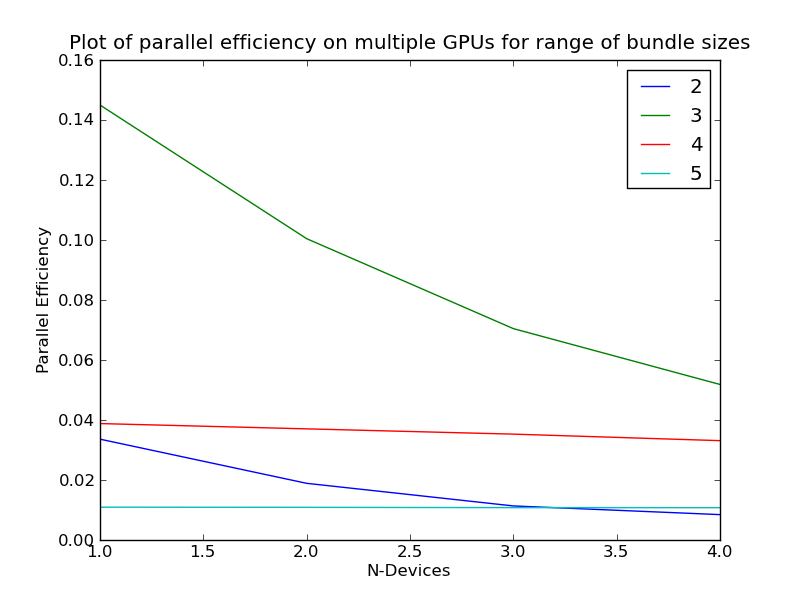
\includegraphics[width=0.45\textwidth,keepaspectratio=true]{cum-results/raw_results/OSB-gpuefficiency.png}\label{fig:GPU-OSB-efficiency}}
\end{figure}

It is clear again that the expected workload is a major factor; the two line bundle 'bottoms out' very quickly, and its speed-up does not grow with additional resourcing. However, the three line bundle reaches a peak at a speed-up of 50.7x faster than CPU, and starts to drop. This echo’s the idea that each workload has a particular 'optimal' processing unit count, and going beyond that count degrades performance.

Looking towards parallel efficiency, strictly speaking each device has 240 PUs\footnote{Each device is a Tesla T10 processor, consisting of 32 SMs with 8 CUDA cores (SPs) per SM}, so to be fair to the CPU comparison, this is factored into the efficiency calculation thus; \(E_p=\frac{S_p}{240 \times P}\) where \(P\) is taken as the number of GPUs.

While this looks like an appalling figure, the cost comparison must be made between having 240 PUs sitting on one device in a home computer, versus 240 CPUs stocked in a server farm. 

An interesting development appears in the relative performance between CPU and GPU on five-line bundles; even though GPU is still significantly faster than the CPU implementation, the speedup is an order of magnitude less than for lower size bundles. This is due to the increased utilisation of PSD caching in the CPU version, leading to massively increased memory use but 'reduced' execution time. A future development could be the application of dynamic caching techniques to the GPU implementation.


\section{ISB GPU Performance and Scalability}
\subsection{Runtime vs Bundle Size vs Device Count}
\begin{figure}[h!]
\centering
  \begin{tabularx}{0.5\textwidth}{|c|X|c|c|c|c|}
    \hline
  &CPU time&\multicolumn{4}{|c|}{GPU Count runtime (s)}\\
  N&&1&2&3&4\\\hline
  2&27.625&0.363&0.000&0.000&0.000\\
  3&76.384&0.528&0.497&0.575&0.625\\
  4&225.278&0.940&0.863&0.944&1.020\\
  5&650.274&1.644&1.277&1.266&1.337\\\hline
  \end{tabularx}
\caption{GPU Performance analysis of ISB; execution times against bundle sizes \& device counts}
\label{tab:ISBTable}
\end{figure}

\begin{figure}[h!]
  \centering
  \subfloat[Analysis of Execution speed vs N-GPUs]{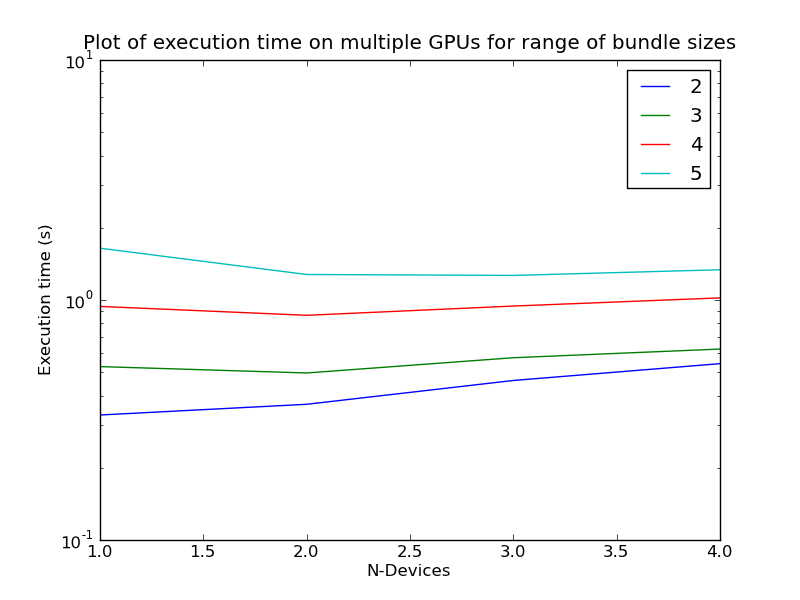
\includegraphics[width=0.5\textwidth,keepaspectratio=true]{cum-results/raw_results/ISB-gpucompare.png}}
  \subfloat[Analysis of Execution speed vs N-Lines]{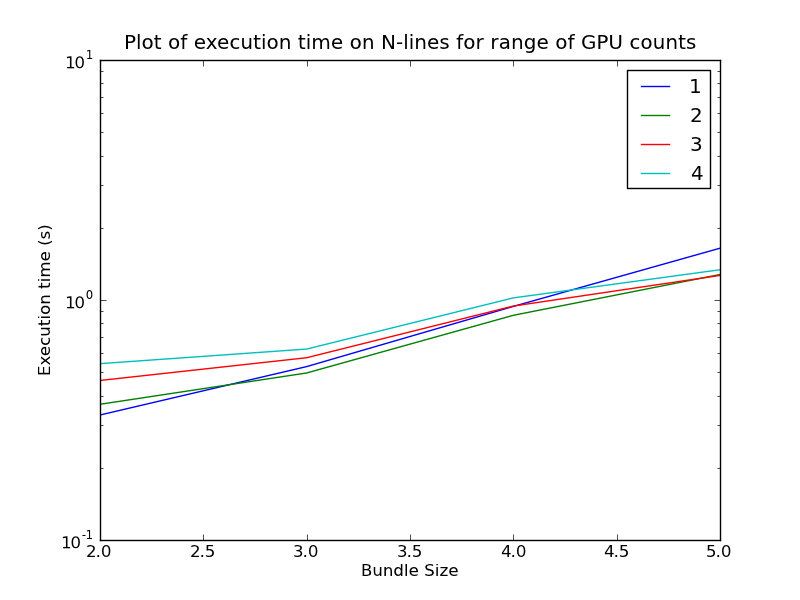
\includegraphics[width=0.5\textwidth,keepaspectratio=true]{cum-results/raw_results/ISB-linecompare.png}}
  \\
  \caption{Graphs of ISB Multi-GPU performance}
  \label{fig:GPU-ISB-multicomp}
\end{figure}

The results of ISB are particularly interesting; looking specifically at the multi-device behaviour of the two-line bundle, its clear that using more devices for this small workload actually makes execution much much worse. This can again be explained as an artefact of CUDA's memory transfer costs. In-fact in ISB, there is very little justification for applying multiple devices to this problem. This pattern of behaviour is also indicated in the larger-line versions, but shows a 'sweet spot' at two devices.

\subsection{Relative Speed-up}
Applying the same caveats as with OSB, GPU ISB performance relative to CPU execution can be inferred. 
\begin{figure}[h!]
\centering
\subfloat[ISB Parallel Speedup]{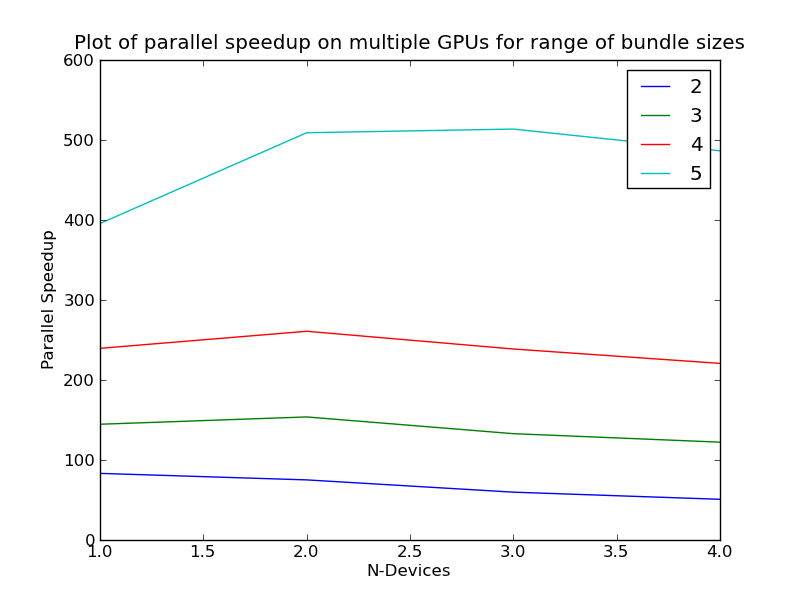
\includegraphics[width=0.45\textwidth,keepaspectratio=true]{cum-results/raw_results/ISB-gpuspeedup.png} \label{fig:GPU-ISB-speedup}}
\subfloat[ISB Parallel Efficiency]{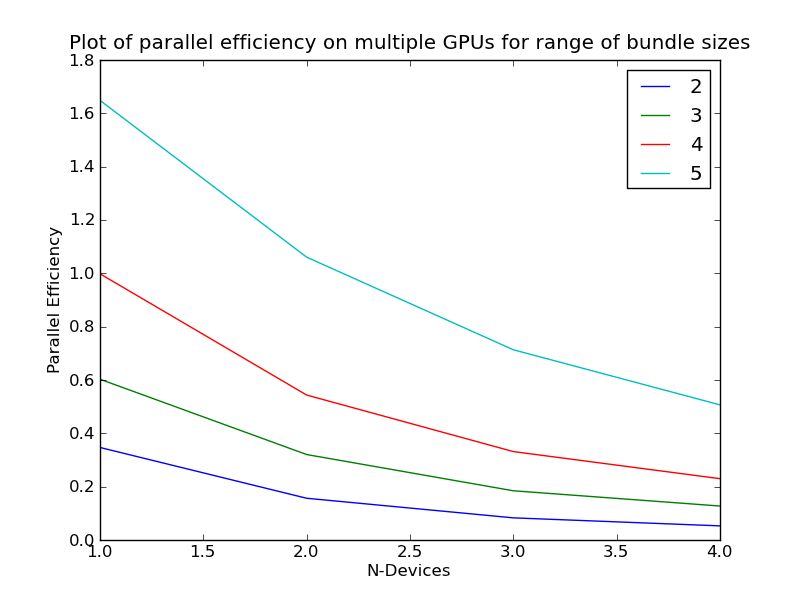
\includegraphics[width=0.45\textwidth,keepaspectratio=true]{cum-results/raw_results/ISB-gpuefficiency.png}\label{fig:GPU-ISB-efficiency}}
\end{figure}
Counter to OSB, The parallel efficiency curves demonstrated are much more stable. This stability is echoed in the more consistent curves of both the speedup graph and N-line execution speed. From this it can be inferred again that there is a partial 'sweet spot' at two devices, but this is not nearly as pronounced.

What is impressive is the level of speedup attained by ISB compared to OSB; since ISB optimises the entire bundle in parallel, there are far fewer memory transfers, meaning that there is less associated cost per kernel invocation. Even comparing like-for-like, the maximum four line speed-up in ISB is almost five times that of OSB's (238x), and ISB's speed-up appears to be tied, at least in this lower-end of the bundle size scale, to the number of lines. Again, this is due to the internal iterative nature of GPU ISB; the more lines there are, the more work each kernel does, the lower proportion of time taken by memory transfers, leading to greatly improved performance over CPU-bound implementations.

